%! TEX root = main.tex 

\graphicspath{{00_Images/01_chapter/}}

\chapter{Review of Fundamentals}
\label{ch:rev}

\section{Basics}

The acoustical operating principle determines the type of sensor used. For example, a pressure gradient transducer detects sound based on pressure differences. The sensitivity of a sensor is defined as the minimum value of pressure that can be detected at each frequency. In electrical systems, circuit elements map current to voltage, usually expressed as:
\[
V = f(I)
\]

\paragraph{Basic Quantities}
\[
I = [A] = \left[\frac{C}{s}\right], \qquad
V = [V] = \left[\frac{J}{C}\right], \qquad
P = I \cdot V = \left[\frac{C}{s} \cdot \frac{J}{C}\right] = \left[\frac{J}{s}\right] = [W]
\]

\subsection{Graph-Theory View of Circuits}

In circuit analysis, an electrical network can be described using basic concepts from graph theory. This representation is useful for precisely defining nodes, branches and loops.

\paragraph{Graph of a circuit} A circuit can be modeled as a graph \( \mathcal{G} = (\mathcal{N}, \mathcal{B}) \), where:

\begin{itemize}
    \item \( \mathcal{N} \) is the set of nodes;
    \item \( \mathcal{B} \) is the set of branches.
\end{itemize}

Elements (resistors, sources, capacitors, etc.) are associated with branches, while electrical interconnections (wires/connection points) define nodes.

\paragraph{Node} A node is a set of points connected by ideal conductors (wires); therefore, all points in the same node share the same electric potential. One node is typically chosen as the reference node (ground) and all node voltages are measured with respect to it.

\paragraph{Branch} A branch is a connection between two nodes that contains one (or more) circuit elements. Each branch is characterized by a branch current \(i_b(t)\) and a branch voltage \(v_b(t)\), defined according to a chosen reference direction and polarity.

\paragraph{Path and loop} A path is an ordered sequence of branches that connects two nodes. A loop is a path that starts and ends at the same node without repeating nodes.

\paragraph{Closed loop (mesh)} A closed loop is any loop in the circuit graph. In planar circuits, a mesh is a closed loop that does not enclose any other loops (i.e., an elementary loop). 

\begin{figure}[!htb]
    \centering
    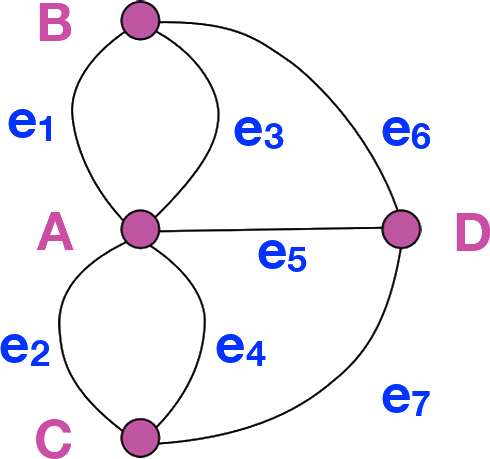
\includegraphics[width=0.4\linewidth]{Graphs.png}
    \caption{Example of circuit graph representation. The vertices \(A,B,C,D\) are the nodes of the graph. The edges \(e_1,\dots,e_7\) are the branches (each branch can represent one circuit element or a series of elements between two nodes). In particular, \(e_1\) and \(e_3\) are two distinct branches connecting the same pair of nodes \((A,B)\) (parallel connection) and they form a closed loop \(A \rightarrow B \rightarrow A\). Similarly, \(e_2\) and \(e_4\) connect \((A,C)\) and form the loop \(A \rightarrow C \rightarrow A\). Other examples of closed loops are \(A \rightarrow B \rightarrow D \rightarrow A\), obtained by traversing \(\{e_3, e_6, e_5\}\) and \(A \rightarrow C \rightarrow D \rightarrow A\), obtained by traversing \(\{e_4, e_7, e_5\}\)}
    \label{fig:graph_example}
\end{figure}

\subsection{Kirchhoff’s Laws}

\paragraph{Current Law (KCL)} For any node with \( N \) branches, the sum of currents flowing into the node is zero.
\[
\sum_{n=1}^{N} i_n = 0
\]

\paragraph{Voltage Law (KVL)} For any closed loop in a circuit, the sum of voltages is zero.
\[
\sum_{n=1}^{N} v_n = 0
\]

\begin{figure}[!htb]
    \centering
    \subfloat[KCL \( \rightarrow I_1 + I_2 = I_3 + I_4 + I_5 \)]{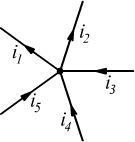
\includegraphics[height=0.23\textheight]{KCL.png}}\hfill
    \subfloat[KVL \( \rightarrow E_1 + E_2 - E_3 = V_1 + V_2 + V_3 + V_4 \)]{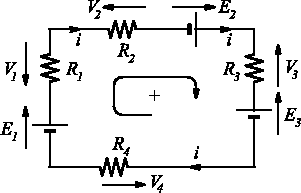
\includegraphics[height=0.23\textheight]{KVL.png}}
    \caption{Illustration of the Kirchhoff's laws}
\end{figure}

\section{Basics Elements}

\subsection{Passive Components}
\label{ssc:121}

\paragraph{Resistor} A resistor \( R \) is expressed in Ohms \si{\ohm}. The current-voltage relation is:
\[
v_R(t) = R i_R(t)
\]
Typical values span from a few \si{\ohm} to several \si{\mega\ohm}. Common SI multipliers are:
\[
\SI{1}{\kilo\ohm}= \SI{e3}{\ohm},
\qquad
\SI{1}{\mega\ohm}= \SI{e6}{\ohm}
\]

\paragraph{Conductance} A conductance \( G \) is expressed in Siemens \si{\siemens} (historically also called mho) and is the inverse of resistance:
\[
G = \frac{1}{R}\qquad\Rightarrow\qquad \si{\siemens}=\si{\ohm^{-1}}
\]
The current-voltage relation is:
\[
i_G(t) = G v_G(t)
\qquad \Leftrightarrow \qquad
v_G(t) = \frac{1}{G} i_G(t)
\]
In this course, the symbol used for conductance is the circled-resistor one to avoid confusion and to make it easier to recognize.

\paragraph{Inductor} An inductor \( L \) is expressed in Henrys \si{\henry}. The current-voltage relation is:
\[
v_L(t) = L\frac{d i_L(t)}{dt}
\qquad \Rightarrow \qquad
i_L(t) = i_L(0) + \frac{1}{L}\int_{0}^{t} v_L(\tau)\, d\tau
\]
In electronics, common values are typically from \SI{1}{\nano\henry} to \SI{1}{\milli\henry} (sometimes higher in filters and power stages):
\[
\SI{1}{\nano\henry}= \SI{e-9}{\henry},
\qquad
\SI{1}{\micro\henry}= \SI{e-6}{\henry},
\qquad
\SI{1}{\milli\henry}= \SI{e-3}{\henry}
\]
In electroacoustics and power applications, inductors are often larger (e.g., \SIrange{1}{10}{\milli\henry} up to \SI{1}{\henry} and beyond, depending on the system). Inductors can also be represented with two parallel lines next to the usual coil symbol; this typically indicates a magnetic core (e.g., ferromagnetic core), i.e., a different construction compared to an air-core inductor.

\paragraph{Capacitor} A capacitor \( C \) is expressed in Farads \si{\farad}. The current-voltage relation is:
\[
i_C(t) = C\frac{d v_C(t)}{dt}
\qquad \Rightarrow \qquad
v_C(t) = v_C(0) + \frac{1}{C}\int_{0}^{t} i_C(\tau)\, d\tau
\]
In practice, capacitor values are commonly specified using submultipliers, especially from pico- to milli-:
\[
\SI{1}{\pico\farad}= \SI{e-12}{\farad},
\qquad
\SI{1}{\nano\farad}= \SI{e-9}{\farad},
\qquad
\SI{1}{\micro\farad}= \SI{e-6}{\farad},
\qquad
\SI{1}{\milli\farad}= \SI{e-3}{\farad}
\]
A capacitor can be polarized, meaning it must be connected with the correct polarity (orientation) in the circuit.

\paragraph{Notes} In audio (and more generally for sinusoidal steady-state signals), the voltage and current of capacitors and inductors are \SI{90}{\degree} out of phase:
\begin{itemize}
    \item for a capacitor, the current leads the voltage by \SI{90}{\degree};
    \item for an inductor, the voltage leads the current by \SI{90}{\degree}.
\end{itemize}

\begin{figure}[!htb]
    \centering
    \subfloat[Resistor]{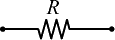
\includegraphics[height=0.05\textheight]{Resistor.png}}\hfill
    \subfloat[Conductance]{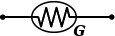
\includegraphics[height=0.05\textheight]{Conductance.png}}\hfill
    \subfloat[Capacitor]{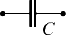
\includegraphics[height=0.05\textheight]{Capacitor.png}}\hfill
    \subfloat[Inductor]{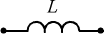
\includegraphics[height=0.05\textheight]{Inductor.png}}
    \caption{Model of passive elements}
\end{figure}

\subsection{Active Components}

\paragraph{Voltage Generator}

A voltage generator provides a prescribed voltage \(V_s\). The resulting current \(I_s\) depends on the connected circuit (load). A voltage source is typically drawn as:

\begin{itemize}
    \item a circle with \(+\) and \(-\) to indicate the voltage polarity;
    \item a battery symbol (stacked long/short plates) for DC supplies;
    \item a circle with a vertical line (often used to denote an ideal DC voltage source in a compact way);
    \item a circle with a sinusoid for AC (sinusoidal) sources;
    \item power pins/nets such as \(V_{DD}\) and \(\mathrm{GND}\), used as connection labels in schematics (especially in electronics).
\end{itemize}

In this course, the preferred symbol is the circle with a vertical line.

\paragraph{Current Generator} A current generator provides a prescribed current \(I_s\). The resulting voltage \(V_s\) depends on the connected circuit. A current source is typically drawn as:

\begin{itemize}
    \item a circle with an arrow indicating the current direction;
    \item a circle with a horizontal line (compact notation for an ideal current source);
    \item a circle with a sinusoid and arrow for AC current sources;
    \item in some schematics, net labels/pins may be used to indicate a bias or reference current connection.
\end{itemize}

In this course, the preferred symbol is the circle with a horizontal line. In drawings, it is often accompanied by an arrow to make the direction explicit.

\begin{figure}[!htb]
    \centering
    \subfloat[Voltage]{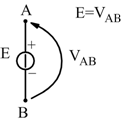
\includegraphics[height=0.12\textheight]{Volt_Gen.png}}\hspace{0.5cm}
    \subfloat[Current]{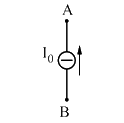
\includegraphics[height=0.12\textheight]{Curr_Gen.png}}
    \caption{Generators models}
\end{figure}

\paragraph{Controlled Generators} In a controlled (dependent) generator, the output voltage or current depends on a controlling variable (voltage or current) defined elsewhere in the circuit. Controlled sources are commonly drawn with a diamond (squared) shape, often including an acronym.

\begin{itemize}
    \item VCVS (Voltage-Controlled Voltage Source): the output voltage depends on a control voltage,
    \[
    v_o(t) = A v_c(t)
    \]
    where \(A\) is a dimensionless gain.
    \item VCCS (Voltage-Controlled Current Source): the output current depends on a control voltage,
    \[
    i_o(t) = g v_c(t)
    \]
    where \(g\) is a transconductance, expressed in \si{\siemens}.
    \item CCVS (Current-Controlled Voltage Source): the output voltage depends on a control current,
    \[
    v_o(t) = r i_c(t)
    \]
    where \(r\) is a transresistance, expressed in \si{\ohm}.
    \item CCCS (Current-Controlled Current Source): the output current depends on a control current,
    \[
    i_o(t) = \beta i_c(t)
    \]
    where \(\beta\) is a dimensionless gain.
\end{itemize}

The output polarity (for voltage sources) is indicated with \(+\) and \(-\) on the diamond, while the output direction (for current sources) is indicated with an arrow. The diamond often contains the acronym (e.g., \(\mathrm{VCVS}\), \(\mathrm{VCCS}\)) or the proportionality (e.g., \(A v_c\), \(g v_c\), \(\beta i_c\)).

\section{Basic Circuits}
\label{sec:simplydiveders}

First, let's introduce what solving a circuit means. It means to determine all the unknown electrical quantities in the network: in particular, the voltage across and the current through every element, consistently with the chosen reference directions (polarities and current arrows). In practice, this is done by writing the circuit equations (e.g., Kirchhoff’s laws and the element constitutive relations) and computing node voltages, branch currents and any requested output quantities.

\subsection{Voltage Divider}

\begin{figure}[!htb]
    \centering
    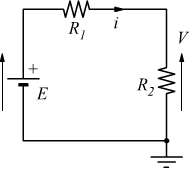
\includegraphics[width=0.3\linewidth]{Volt_Div.png}
    \caption{Voltage divider}
    \label{fig:volt_div}
\end{figure}

A voltage divider is made of an ideal voltage source providing the input voltage \(V_{IN}(t)\) and two resistors \(R_1\) and \(R_2\) connected in series. The same current \(i(t)\) flows through both resistors; the output voltage is typically taken across \(R_2\) and denoted as \(V_{OUT}(t)\). From Kirchhoff’s laws:
\[
V_{IN}(t) = V_{R_1}(t) + V_{R_2}(t),
\qquad
i_{R_1}(t) = i_{R_2}(t) = i(t)
\]
Using Ohm’s law:
\[
V_{R_1}(t) = i(t)R_1,
\qquad
V_{R_2}(t) = i(t)R_2
\]
Thus:
\[
V_{IN}(t) = i(t)\left(R_1 + R_2\right)
\]
Defining the equivalent resistance \(R_{eq} = R_1 + R_2\)
\[
i(t) = \frac{V_{IN}(t)}{R_{eq}}
\]

\paragraph{Meaning of the voltage divider} The voltage divider distributes the input voltage among the series resistors proportionally to their resistance values. If the input is \(V_{IN}(t)\), then each resistor drops a fraction of it:
\[
V_{R_1}(t) = \frac{R_1}{R_1 + R_2}V_{IN}(t),
\qquad
V_{R_2}(t) = \frac{R_2}{R_1 + R_2}V_{IN}(t)
\]
Therefore, the output voltage taken across \(R_2\) is:
\[
V_{OUT}(t) = V_{R_2}(t) = \frac{R_2}{R_1 + R_2}V_{IN}(t)
\]
so the waveform of the output follows the waveform of the input, scaled by the constant factor \(\tfrac{R_2}{R_1+R_2}\) (assuming an ideal voltage source and no load connected at the output).

\subsection{Current Divider}

\begin{figure}[!htb]
    \centering
    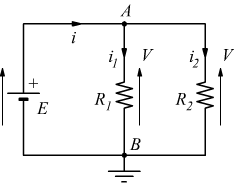
\includegraphics[width=0.3\linewidth]{Curr_Div.png}
    \caption{Current divider (note on the schematic): the picture shows a voltage generator \(E\) feeding two resistors \(R_1\) and \(R_2\) in parallel, therefore it is not a true current-source excitation. In this configuration, the applied voltage is fixed by the source (\(V_{IN}(t)=E\)) and the branch currents are \(I_{R_1}(t)=V_{IN}(t)/R_1\) and \(I_{R_2}(t)=V_{IN}(t)/R_2\), so the total current drawn from the source becomes \(I_{IN}(t)=I_{R_1}(t)+I_{R_2}(t)=V_{IN}(t)(1/R_1+1/R_2)\). In the current-divider problem treated in the text, instead, the excitation is an ideal current source that fixes \(I_{IN}(t)\), while the node voltage \(V_{IN}(t)\) is the unknown and adjusts according to the equivalent resistance \(R_{eq}=R_1\parallel R_2\). The current-divider formulas for the split still hold in both cases because they depend on the parallel condition (same voltage across the branches): with a current source they directly give \(I_{R_1}(t)\) and \(I_{R_2}(t)\) as fractions of the prescribed \(I_{IN}(t)\); with a voltage source they give the ratio between branch currents, while their absolute values are set by the prescribed voltage}
    \label{fig:curr_div}
\end{figure}

A current divider is made of an ideal current source providing the input current \(I_{IN}(t)\) feeding two resistors \(R_1\) and \(R_2\) connected in parallel. The source current splits into the branch currents \(I_{R_1}(t)\) and \(I_{R_2}(t)\). Since the resistors are in parallel, they share the same voltage, denoted as \(V_{IN}(t)\):
\[
V_{IN}(t) = V_{R_1}(t) = V_{R_2}(t)
\]
Using Kirchhoff’s Current Law (KCL) at the top node:
\[
I_{IN}(t) = I_{R_1}(t) + I_{R_2}(t)
\]
Using Ohm’s law on each branch:
\[
V_{R_1}(t) = I_{R_1}(t)R_1,
\qquad
V_{R_2}(t) = I_{R_2}(t)R_2
\]
Since \(V_{R_1}(t) = V_{R_2}(t)\)
\[
I_{R_1}(t)R_1 = I_{R_2}(t)R_2
\qquad \Rightarrow \qquad
I_{R_1}(t) = I_{R_2}(t)\frac{R_2}{R_1}
\]
Substituting into KCL:
\[
I_{IN}(t) = I_{R_2}(t)\left(1+\frac{R_2}{R_1}\right)
= I_{R_2}(t)\frac{R_1+R_2}{R_1}
\]
hence, the branch currents are:
\[
I_{R_2}(t) = I_{IN}(t)\frac{R_1}{R_1+R_2},
\qquad
I_{R_1}(t) = I_{IN}(t)\frac{R_2}{R_1+R_2}
\]

\paragraph{Meaning of the current divider} The current divider distributes the input current between the parallel branches inversely proportional to the resistance values: the smaller resistance carries the larger fraction of the current. The coefficients \(\tfrac{R_1}{R_1+R_2}\) and \(\tfrac{R_2}{R_1+R_2}\) are the current-divider coefficients for \(I_{R_2}(t)\) and \(I_{R_1}(t)\), respectively.

\paragraph{Equivalent resistance and input voltage} The equivalent resistance of two resistors in parallel is:
\[
R_{eq} = R_1 \parallel R_2 = \frac{R_1 R_2}{R_1 + R_2}
\]
Therefore, the voltage across the parallel network (and across each resistor) is:
\[
V_{IN}(t) = V_{R_1}(t) = V_{R_2}(t) = I_{IN}(t)R_{eq}
= I_{IN}(t)\frac{R_1 R_2}{R_1 + R_2}
\]

\section{Circuits as Linear Time-Invariant (LTI) Systems}

Many circuits used in audio and measurement can be modeled as systems that process an input signal into an output signal:
\[
x(t) \longrightarrow \boxed{\text{Circuit/System}} \longrightarrow y(t)
\]
A system is called Linear Time-Invariant (LTI) if it satisfies linearity (superposition) and time invariance. These assumptions are often valid for circuits made of linear elements (\(R\), \(L\), \(C\)) operating in their linear range and with constant parameters. It is often useful to treat circuits as LTI systems, as they have useful properties:

\begin{itemize}
    \item Linearity and superposition principles:
    \[
    y_1(t) = f(x_1(t)), \quad y_2(t) = f(x_2(t))
    \quad \Rightarrow \quad
    f(\alpha x_1(t) + \beta x_2(t)) = \alpha y_1(t) + \beta y_2(t)
    \]
    \item Time invariance principle:
    \[
    y(t) = f(x(t))
    \quad \Rightarrow \quad
    y(t - \tau) = f(x(t - \tau))
    \]
\end{itemize}

\paragraph{Why these properties matter in circuits}

\begin{itemize}
    \item Superposition allows complex excitations to be decomposed into simpler signals, analyzed separately and then summed to obtain the total response (this is essential, for example, when multiple sources are present).
    \item Time invariance guarantees that the circuit behavior does not depend on the absolute time instant: delaying the input produces the same delay at the output. This makes frequency-domain descriptions meaningful and stable over time. 
\end{itemize}

\paragraph{Sinusoidal inputs} A key property of LTI systems is that if the input is a sinusoidal signal, the output will also be a sinusoid of the same frequency, with possibly different amplitude and phase:
\[
x(t) = A_x \sin(\omega t + \phi_x)
\quad \Rightarrow \quad
y(t) = A_y \sin(\omega t + \phi_y),
\qquad \omega_y = \omega_x = \omega
\]
This frequency preservation is crucial: it means the system action on a sinusoid is completely described by two numbers at each frequency: a gain (amplitude scaling) and a phase shift.

\paragraph{Spectrum and Fourier-series viewpoint} Real audio signals are rarely single sinusoids. However, periodic (and, more generally, finite-energy) signals can be represented as sums of sinusoids. For a periodic signal with fundamental frequency \(\omega_0\), the Fourier series can be written (phasor form) as:
\[
x(t) = \sum_{k=-\infty}^{+\infty} X_k e^{j k \omega_0 t}
\]
where each coefficient \(X_k\) contains both amplitude and phase of the \(k\)-th harmonic. The spectrum is the set of these sinusoidal components (often visualized as vertical lines at the present frequencies).

\begin{figure}[!htb]
    \centering
    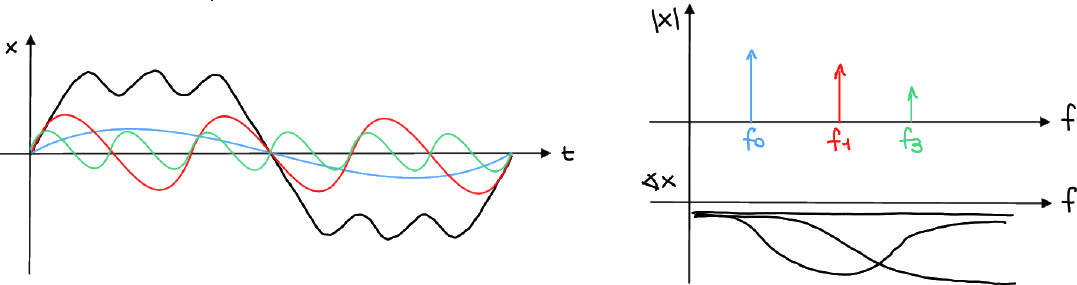
\includegraphics[width=0.7\linewidth]{signal_decomposition.png}
    \caption{Signal decomposition illustration}
    \label{fig:signal_decomposition}
\end{figure}

Because the system is linear, each harmonic is processed independently; because it is time-invariant, each harmonic keeps its frequency. Therefore, for an LTI circuit:
\[
y(t) = \sum_{k=-\infty}^{+\infty} Y_k e^{j k \omega_0 t},
\qquad
Y_k = H(jk\omega_0)X_k
\]
so the transfer function \(H(j\omega)\) tells how each spectral line is scaled and phase-shifted. 

\paragraph{Transfer function} An LTI system can be described in the frequency domain by its transfer function:
\[
H(j\omega) = \frac{Y(j\omega)}{X(j\omega)}
\]
Here \(X(j\omega)\) and \(Y(j\omega)\) represent the Fourier transforms (or the Fourier-series/phasor description at discrete harmonics, for periodic signals). The complex quantity \(H(j\omega)\) encodes:
\[
H(j\omega) = |H(j\omega)|e^{j\angle H(j\omega)}
\]
so at each frequency the circuit applies a magnitude change \(|H(j\omega)|\) and a phase change \(\angle H(j\omega)\). 

\paragraph{Cascaded LTI systems} If multiple LTI blocks are connected in cascade, the overall transfer function is the product of the single transfer functions:
\[
Y(s) = X(s)\cdot \prod_{i=1}^{N} H_i(s),
\qquad\Rightarrow\qquad
H_{\text{tot}}(s)=\prod_{i=1}^{N} H_i(s)
\]
This is very powerful in audio chains
\[
\text{microphone} \rightarrow \text{cable} \rightarrow \text{preamp/mixer} \rightarrow \text{processing} \rightarrow \text{power amplifier} \rightarrow \text{loudspeaker}
\]
Each stage can often be approximated as LTI in its operating range, so the overall response is obtained by multiplying transfer functions. This looks easy because it is ``just a multiplication'', but performing the same operation directly on time-domain waveforms is generally difficult. This is why Bode plots and, later, the pole/zero (canonical) form which turns products into sums in the logarithmic domain are introduced.

\begin{figure}[!htb]
    \centering
    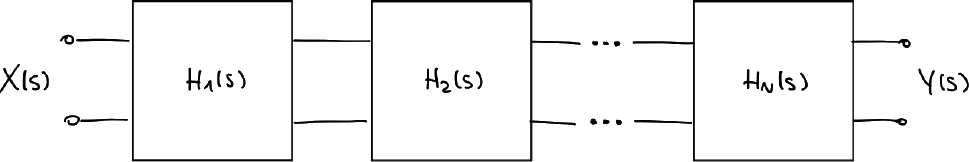
\includegraphics[width=0.7\linewidth]{LTI_cascade_blocks.png}
    \caption{Cascade of LTI systems}
    \label{fig:LTI_cascade}
\end{figure}

\paragraph{Decibels and Bode plots} Since cascaded systems lead to products of transfer functions, it is often convenient to work in decibels because products become sums:
\[
\log_{10}(ab)=\log_{10}(a)+\log_{10}(b)
\]
For voltage (and generally for amplitude ratios)
\[
|H|_{dB} = 20\log_{10}\left(|H(j\omega)|\right)
\]
Bode plots represent magnitude (in dB) and phase (in degrees) versus frequency on a logarithmic axis, enabling simple hand-sketching rules based on poles and zeros (slopes in dB/decade).

\paragraph{Canonical Bode Form} The general transfer function can be expressed in pole/zero form as:
\[
H(s) = K \cdot \frac{N(s)}{D(s)}
= K \cdot \frac{\prod_{i=1}^{N}\left(1+s\tau_{z,i}\right)}{\prod_{j=1}^{M}\left(1+s\tau_{p,j}\right)}
\]
Some filters (e.g., high-pass) include explicit factors of \(s\) in the numerator (or denominator), corresponding to zeros (or poles) at the origin:
\[
H(s)=K s^{n}\frac{\prod_i(1+s\tau_{z,i})}{\prod_j(1+s\tau_{p,j})}
\quad \text{or} \quad
H(s)=K\frac{\prod_i(1+s\tau_{z,i})}{s^{m}\prod_j(1+s\tau_{p,j})}
\]
In frequency response, these become \((j\omega)^n\) or \((j\omega)^{-m}\). 

\begin{itemize}
    \item Each zero at \(f_{z,i}=\tfrac{1}{2\pi\tau_{z,i}}\) increases the magnitude slope by \(+\SI{20}{dB/dec}\) after its corner frequency and introduces a phase lead that transitions from \(\SI{0}{\degree}\) to \(+\SI{90}{\degree}\) around \(f_{z,i}\) (approximately from \(0.1f_{z,i}\) to \(10f_{z,i}\)).
    \item Each pole at \(f_{p,j}=\tfrac{1}{2\pi\tau_{p,j}}\) decreases the magnitude slope by \(-\SI{20}{dB/dec}\) after its corner frequency and introduces a phase lag that transitions from \(\SI{0}{\degree}\) to \(-\SI{90}{\degree}\) around \(f_{p,j}\) (approximately from \(0.1f_{p,j}\) to \(10f_{p,j}\)).
\end{itemize}

\paragraph{Cutoff frequency} For a first-order filter, the cutoff (corner) frequency \(f_c\) is conventionally defined as the frequency at which the magnitude drops to \(\tfrac{1}{\sqrt{2}}\) of its passband value, i.e.,
\[
|H(j\omega_c)|=\frac{1}{\sqrt{2}}|H|_{\text{passband}}
\qquad \Leftrightarrow \qquad
20\log_{10}\!\left(\frac{1}{\sqrt{2}}\right)\approx -\SI{3}{dB}
\]

\paragraph{Why logarithmic plots are so convenient} In linear scale, cascaded systems require multiplying magnitudes:
\[
|H_{\text{tot}}|=|H_1|\cdot|H_2|\cdots|H_N|
\]
In dB scale, the same cascade becomes a sum:
\[
|H_{\text{tot}}|_{dB}=|H_1|_{dB}+|H_2|_{dB}+\cdots+|H_N|_{dB}
\]
which is the key reason why Bode plots simplify both computation and drawing. 

\paragraph{Decade and octave} A decade corresponds to a frequency ratio of \(10\) (e.g., \(\SI{100}{Hz}\rightarrow\SI{1}{kHz}\)); an octave corresponds to a ratio of \(2\) (e.g., \(\SI{500}{Hz}\rightarrow\SI{1}{kHz}\)). A first-order pole/zero produces an asymptotic slope of \(\pm\SI{20}{dB/dec}\) (approximately \(\pm\SI{6}{dB/oct}\)). 

\begin{figure}[!htb]
    \centering
    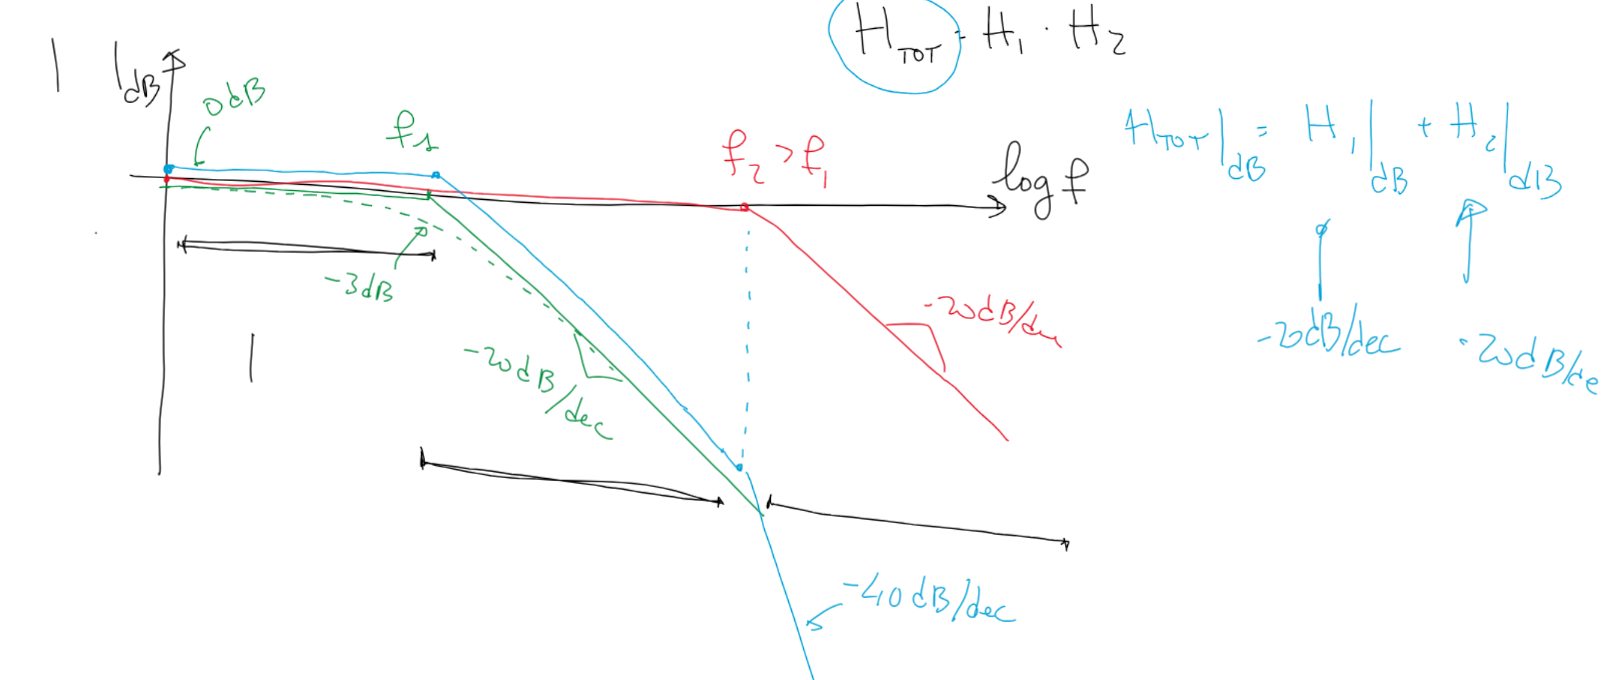
\includegraphics[width=0.7\linewidth]{Example_BodeDiagram.png}
    \caption{Example of a Bode diagram construction on a cascade LTI system (two low pass filter)}
    \label{fig:exampleBode}
\end{figure}

\subsection{RC Low-Pass Filter}

The RC low-pass filter is composed of a resistor \(R\) in series with a capacitor \(C\). The input voltage \(V_{IN}(t)\) (\(E\) in the figure) is applied to the series network and the output voltage \(V_{OUT}(t)\) is typically taken across the capacitor.

\begin{figure}[!htb]
    \centering
    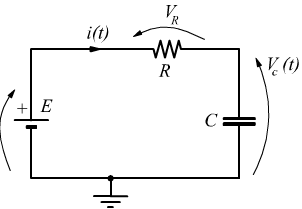
\includegraphics[width=0.5\linewidth]{RC_LPF.png}
    \caption{Low-pass RC filter scheme}
    \label{fig:RC_LPF}
\end{figure}

From Kirchhoff’s laws:
\[
V_{IN}(t) = V_R(t) + V_C(t)
\]
With current-voltage relations:
\[
V_R(t) = I(t)R,
\qquad
V_C(t) = \frac{1}{C}\int_{0}^{t} I(\tau)\, d\tau
\]
Differentiating the KVL equation with respect to time removes the integral and yields a differential equation.
\[
\frac{dV_{IN}(t)}{dt} = R\frac{dI(t)}{dt} + \frac{1}{C}I(t)
\]
Solving such differential equations directly is possible, but it requires careful handling of derivatives/integrals, initial conditions and piecewise inputs. For systematic circuit analysis (especially for filters), it is more convenient to use the Laplace transform, which converts derivatives and integrals into algebraic factors in \(s\). Instead of solving the differential equation directly, the Laplace Transform is used (for causal signals, typically integrating from \(0\) to \(+\infty\)):
\[
\mathcal{L}\{f(t)\} = F(s) = \int_{0}^{+\infty} f(t) e^{-st}\, dt,
\qquad s\in\mathbb{C}
\]
In this course, lowercase letters denote time-domain quantities (e.g., \(v(t)\), \(i(t)\)) and the corresponding uppercase letters denote Laplace-domain quantities (e.g., \(V(s)\), \(I(s)\)). Applying Laplace to the capacitor relation:
\[
v_C(t) = \frac{1}{C}\int_{0}^{t} i(\tau)\, d\tau
\qquad \xrightarrow{\ \mathcal{L}\ }\qquad
V_C(s) = \frac{1}{sC} I(s)
\]
which immediately provides the capacitor impedance:
\[
Z_C(s) = \frac{V_C(s)}{I(s)} = \frac{1}{sC}
\]
Similarly, in the Laplace domain impedances (all expressed in \si{\ohm}) for the basic elements are defined as follows
\[
Z_R = R,
\qquad
Z_L(s) = sL,
\qquad
Z_C(s) = \frac{1}{sC}
\]
Because impedances have the same unit as resistance, the same algebraic divider rules introduced in section \ref{sec:simplydiveders} (voltage divider/current divider) can be applied, now in the \(s\)-domain. Using the impedance voltage divider for the RC series network (output across the capacitor):
\[
V_{OUT}(s) = V_{IN}(s)\frac{Z_C(s)}{Z_R + Z_C(s)}
\qquad \Rightarrow \qquad
H(s) = \frac{V_{OUT}(s)}{V_{IN}(s)} = \frac{Z_C(s)}{Z_R + Z_C(s)}
\]
Substituting \(Z_R=R\) and \(Z_C(s)=\tfrac{1}{sC}\):
\[
H(s) = \frac{\tfrac{1}{sC}}{R + \tfrac{1}{sC}}
\qquad \Rightarrow \qquad
H(s) = \frac{1}{1+sRC}
\]

\begin{figure}[!htb]
    \centering
    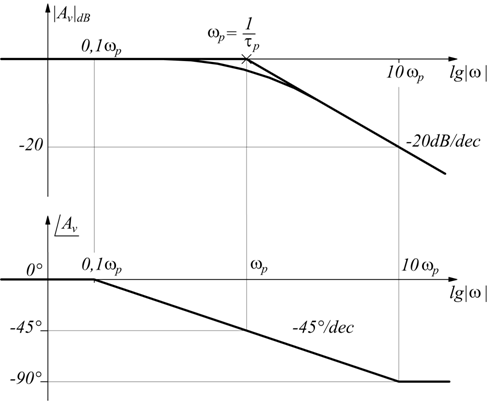
\includegraphics[width=0.7\linewidth]{Bode_LowPass.png}
    \caption{Bode diagram of a low pass filter}
    \label{fig:BodeLP}
\end{figure}

\paragraph{Impedance viewpoint (frequency intuition)} The capacitor impedance decreases with frequency:
\[
|Z_C(j\omega)|=\left|\frac{1}{j\omega C}\right|=\frac{1}{\omega C}
\]
Therefore:

\begin{itemize}
    \item for low frequencies (\(\omega \ll \omega_c\)): \(|Z_C|\) is large (almost open circuit) \(\Rightarrow V_{OUT}\approx V_{IN}\);
    \item for high frequencies (\(\omega \gg \omega_c\)): \(|Z_C|\) is small (almost short circuit) \(\Rightarrow V_{OUT}\approx 0\).
\end{itemize}

For a general audio signal (sum of many sinusoids), low-frequency components pass almost unchanged, while high-frequency components are strongly attenuated; the output spectrum is the input spectrum multiplied by \(|H(j\omega)|\) at each frequency. 

\subsection{RC High-Pass Filter}

%\begin{figure}[H]
%    \centering
%    \includegraphics[width=\linewidth]{RC_HPF_LT.png}
%    \caption{RC HPF scheme}
%    \label{fig:RC_HPF_LT}
%\end{figure}

Now consider the complementary case, with capacitor in series and resistor across the output (output across \(R\)). Using impedances:
\[
V_{OUT}(s) = Z_R  I(s)
\quad \Rightarrow \quad
V_{OUT}(s) = Z_R \cdot \frac{V_{IN}(s)}{Z_R+Z_C(s)}
\]
Thus, the transfer function is:
\[
H(s) = \frac{V_{OUT}(s)}{V_{IN}(s)}
= \frac{Z_R}{Z_R + Z_C(s)}
= \frac{R}{R + \tfrac{1}{sC}}
\quad \Rightarrow \quad
H(s) = \frac{sRC}{1 + sRC}
\]
This is a high-pass filter: it has a zero at the origin (the factor \(s\) in the numerator) and a pole at \(\omega_c=\tfrac{1}{RC}\). In canonical Bode form:
\[
H(s)=\frac{sRC}{1+sRC}= (sRC)\cdot \frac{1}{1+sRC}
\]
Therefore, in magnitude Bode terms:

\begin{itemize}
    \item the factor \((j\omega)\) contributes \(+\SI{20}{dB/dec}\);
    \item the pole factor \(\tfrac{1}{1+j\omega RC}\) contributes a \(-\SI{20}{dB/dec}\) slope after \(\omega_c\);
    \item the overall result is a rising response at low frequencies that flattens to \(\approx \SI{0}{dB}\) at high frequencies.
\end{itemize}

A direct computation is obtained by evaluating \(H(j\omega)\):
\[
H(j\omega)=\frac{j\omega RC}{1+j\omega RC},
\qquad
|H(j\omega)|=\frac{\omega RC}{\sqrt{1+(\omega RC)^2}},
\qquad
\angle H(j\omega)=\frac{\pi}{2}-\arctan(\omega RC)
\]
These expressions match the canonical Bode interpretation (zero at the origin + pole at \(\omega_c\)).

\begin{figure}[!htb]
    \centering
    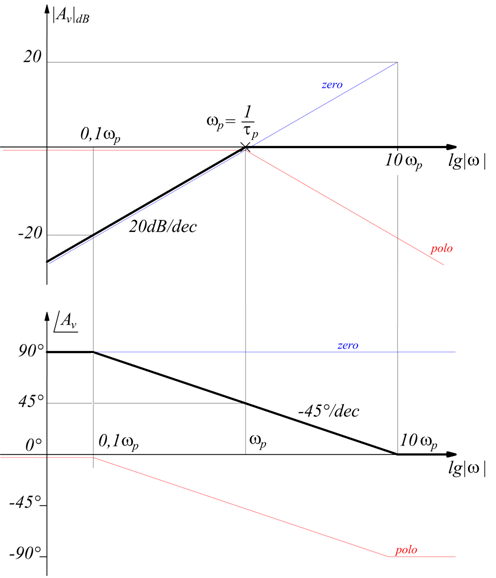
\includegraphics[width=0.7\linewidth]{Bode_HighPass.png}
    \caption{Bode diagram of a high pass filter}
    \label{fig:BodeHP}
\end{figure}

\subsection{Band-Pass Filter}

A band-pass response can be obtained conceptually by combining a high-pass behavior at low frequencies with a low-pass behavior at high frequencies (e.g., cascading an RC high-pass with an RC low-pass, or using RLC topologies). In Bode magnitude, this corresponds to a slope that rises up to a mid-band, then falls after a second corner frequency.

\begin{figure}[!htb]
    \centering
    \subfloat[Simplified scheme]{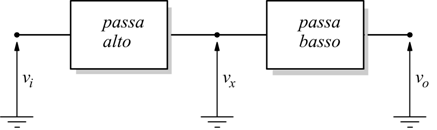
\includegraphics[width=0.7\linewidth]{BandPass_Brutto.png}}
    \\
    \subfloat[Bode diagram]{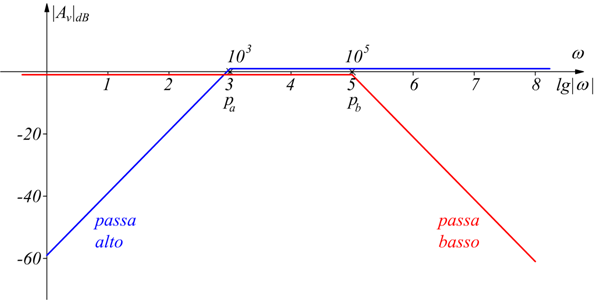
\includegraphics[width=0.7\linewidth]{Bode_BandPass.png}}
    \caption{Band pass filter}
    \label{fig:BPF}
\end{figure}

\paragraph{Note} More information and examples/exercises on this entire part of the course are available on following websites (unfortunately only in Italian):

\begin{itemize}
    \item \href{https://www.edutecnica.it/elettrotecnica.htm}{Edutecnica-Elettrotecnica}.
    \item \href{https://www.edutecnica.it/elettronica.htm}{Edutecnica-Elettronica}.
\end{itemize} 

\section{Audio Signals}

Audio systems can be described as signal-processing chains where an input (typically generated by a source) is transported, conditioned and finally delivered to a load (the application). From an electrical viewpoint, each block can often be modeled (at first order) as an LTI system characterized by impedances and transfer functions. A typical audio chain is:
\[
\text{Source} \rightarrow \text{Preamp} \rightarrow \text{Processing/Mixer} \rightarrow \text{Power Amp} \rightarrow \text{Load (Loudspeaker)}
\]
In words:

\begin{itemize}
    \item the source produces an audio signal (e.g., microphone capsule, pickup, line device);
    \item the pre-amplifier raises the signal to a usable level while minimizing loading effects;
    \item processing/mixing applies equalization, filtering, dynamics, routing and level control (often with an optional digital branch);
    \item the power amplifier provides the current and voltage needed to drive the load;
    \item the load converts electrical power into another form, typically acoustic power (loudspeaker) or a monitored signal (headphones, measurement input).
\end{itemize}

\paragraph{Sources and loads: the most critical elements} In practice, the most difficult parts of the chain to represent with simple electrical models are the sources (because they include an electromechanical transduction mechanism and internal constraints) and the loads, especially loudspeakers (because their impedance and behavior depend on frequency, mechanics and acoustics). For this reason, the detailed electrical modeling and transduction mechanisms of microphones and loudspeakers will be treated in Module 2. In this module, we will use standard simplified representations of these elements using basic components (\(R\), \(L\), \(C\)).

\paragraph{Standard simplified models used in this course} Depending on the device and the frequency range of interest, real electroacoustic components can be approximated as:

\begin{itemize}
    \item Resistive behavior: an ideal load or a simplified loudspeaker model is sometimes approximated as a resistance (e.g., \(\SI{8}{\ohm}\) nominal load), useful for basic power and divider reasoning.
    \item Capacitive behavior: some sensors and inputs (e.g., condenser microphone capsule, piezo elements, cable capacitance, amplifier inputs) may be approximated as capacitive, especially when the dominant effect is charge/voltage storage.
    \item Inductive behavior: coils and electromagnets (e.g., voice coils, transformers) often show inductive behavior, especially at mid/high frequency where \(Z_L=j\omega L\) increases with \(\omega\).
\end{itemize}

\begin{figure}[!htb]
    \centering
    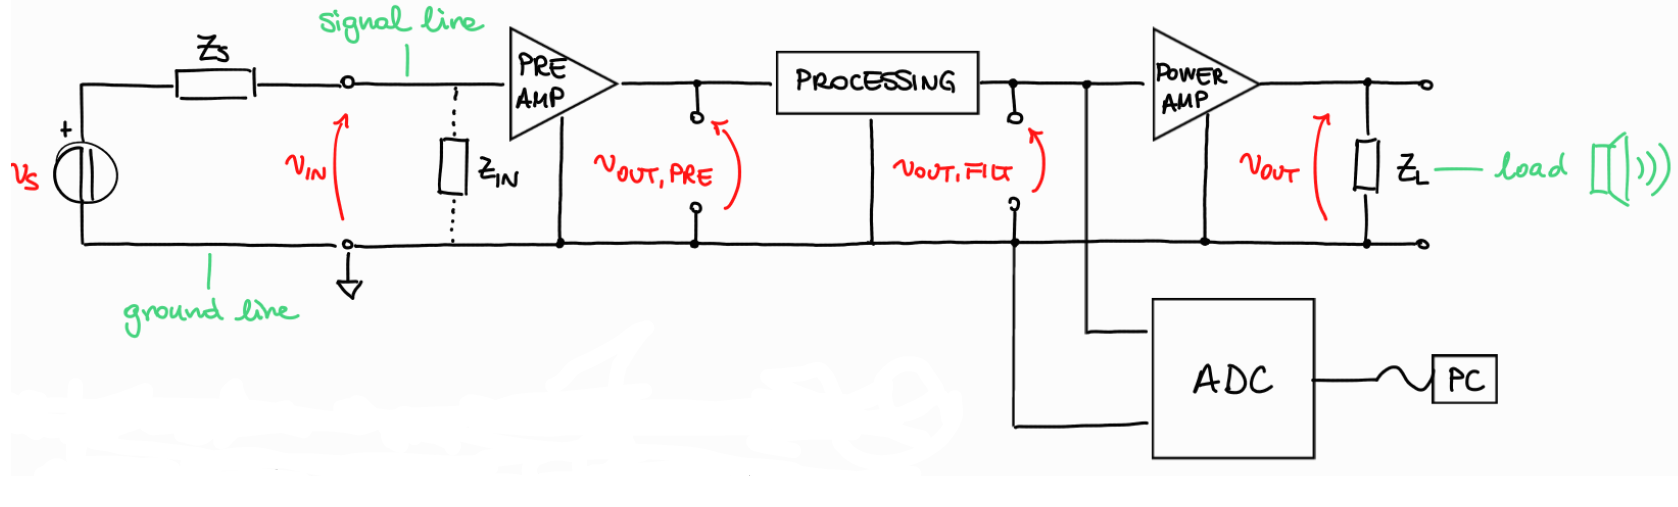
\includegraphics[width=0.85\linewidth]{Audio_Signal_Path.png}
    \caption{Example of an audio signal chain and its electrical interpretation. The source is modeled as an ideal generator \(v_s(t)\) with series impedance \(Z_s\); the signal line carries the input voltage \(v_{IN}(t)\) to the preamplifier, whose input impedance \(Z_{IN}\) should be high to minimize loading (\(v_{IN}=v_s\tfrac{Z_{IN}}{Z_s+Z_{IN}}\)). The preamp output \(v_{OUT,\mathrm{PRE}}(t)\) is then processed (filtering/mixing) to obtain \(v_{OUT,\mathrm{FIL}}(t)\), which drives the power amplifier and produces the final output voltage \(v_{OUT}(t)\) on the load \(Z_L\) (e.g., loudspeaker). The diagram also shows an optional digital branch where the signal is converted by an ADC and sent to a PC for digital processing/recording}
    \label{fig:source_load_divider}
\end{figure}

\subsection{Loading, Input Impedance and Pre-amplification}

A key role of the pre-amplification stage is to provide initial voltage gain and level control, bringing the signal into a correct operating range for the following stages. Equally important, the preamp must avoid loading the source: many audio sources are sensitive to the impedance connected to them and their delivered voltage can drop if the input impedance is too low.

\paragraph{Voltage transfer with source and input impedances} A common (and very useful) model is:

\begin{itemize}
    \item the source is represented by an ideal voltage generator \(v_s(t)\) in series with a source impedance \(Z_s\);
    \item the receiving stage (preamp input) is represented by an input impedance \(Z_{IN}\).
\end{itemize}

The voltage actually available at the input of the next stage is given by the impedance voltage divider:
\[
v_{IN}(t) = v_s(t)\frac{Z_{IN}}{Z_s + Z_{IN}}
\]
If \(Z_{IN}\) is much larger than \(Z_s\), then the divider ratio approaches \(1\), hence:
\[
\lim_{Z_{IN}\to\infty} v_{IN}(t) = v_s(t)
\]
This shows a central design rule in audio interfaces:
\[
Z_{IN} \gg Z_s \quad \Rightarrow \quad \text{minimal loading and maximal voltage transfer}
\]

\paragraph{What this implies in the audio chain}

\begin{itemize}
    \item For voltage-driven interconnections (typical of line-level and microphone preamps), we generally want high input impedance so the source voltage is preserved.
    \item If \(Z_{IN}\) is not sufficiently high, part of the signal is lost across \(Z_s\) and the frequency response can be altered if \(Z_s\) and \(Z_{IN}\) are frequency-dependent (for example due to capacitive or inductive effects).
\end{itemize}
